\documentclass[../../thesis.tex]{subfiles}
  \begin{document}
    \begin{figure}[tb]
      \centering
      \pgfdeclarelayer{bg}    % declare background layer
      \pgfdeclarelayer{bbg}    % declare backbackground layer
      \pgfsetlayers{bbg,bg,main}  % set the order of the layers (main is the standard layer)
      \tikzsetnextfilename{lad}
      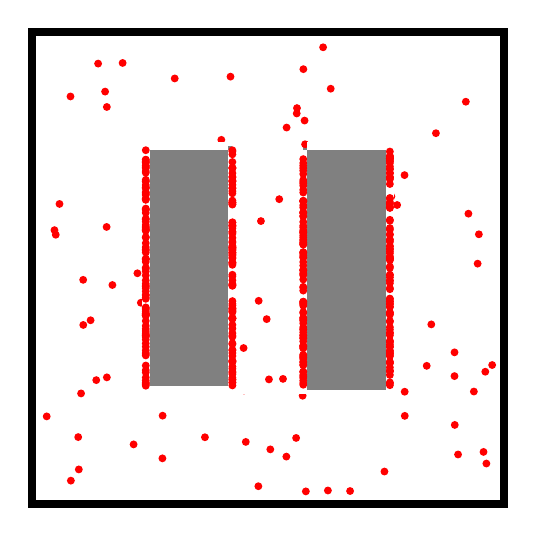
\begin{tikzpicture}
        \draw[color=black, line width=1mm] (-3,-3) rectangle (3,3);
        \draw[color=gray, line width=1mm] (-1.5,-1.5)--(-.5,-1.5)--(-.5,1.5)--(-1.5,1.5);
        \draw[color=gray, line width=1mm] (1.5,-1.5)--(.5,-1.5)--(.5,1.5)--(1.5,1.5);
        \foreach \x in {1,...,100}{
          \fill[red] (rand*2.9,rand*2.9) circle(0.5mm);
        }
        \fill[gray] (-1.5,-1.5) rectangle (-0.5,1.5);
        \fill[gray] (.5,-1.5) rectangle (1.5,1.5);
        \fill[white] (-1.6,-1.5) rectangle (-1.5,1.5);
        \fill[white] (-0.5,-1.5) rectangle (-0.4,1.5);
        \fill[white] (1.6,-1.5) rectangle (1.5,1.5);
        \fill[white] (0.4,-1.5) rectangle (0.5,1.5);
        \fill[white] (-1.5,-1.5) rectangle (-0.5,-1.6);
        \fill[white] (-1.5,1.5) rectangle (-0.5,1.6);
        \fill[white] (0.5,-1.5) rectangle (-1.5,-1.6);
        \fill[white] (0.5,1.5) rectangle (1.5,1.6);
        \foreach \x in {1,...,100}{
          \fill[red] (-0.45,rand*1.5) circle(0.5mm);
          \fill[red] (-1.55,rand*1.5) circle(0.5mm);
          \fill[red] (0.45,rand*1.5) circle(0.5mm);
          \fill[red] (1.55,rand*1.5) circle(0.5mm);
        }
      \end{tikzpicture}
      \caption{Illustration of the ALD process to go along with the explanations in \cref{subsec:ald}.}
      \label{fig:ald}
  \end{figure}
\end{document}
